\subsection*{Questions 1 through 3}

\colorbox{Cerulean!25}{ \parbox{\textwidth}{
    \textbf{\textit{\underline{Question}}}:
\textit{\begin{enumerate}
    \item Label and interpret the model ingredients properly.
    \item Discretise the idiosyncratic productivity process by the Tauchen method using 2 grid points
on one standard deviation range.
    \item Characterise the individual (probabilistic) labour supply decision analytically.
\end{enumerate}}}}\\

% \begin{aligned}
%\\
%  \\
% \\
% 
% \end{aligned}

The value functions are:
\begin{subequations}
    \begin{align}
          V_t(a, h, z) =\int \max \left\{W_t(a, h, z)+\xi_{W t}, N_t(a, h, z)+\xi_{N t}\right\} d G\left(\xi_{s t} ; \xi\right) 
    \end{align}
    and 
    \begin{align}
         S_t(a, h, z) =\int \max \left\{\varphi W_t(a, h, z)+(1-\varphi) N_t(a, h, z)-\phi+\xi_{W t}, N_t(a, h, z)+\xi_{N t}\right\} d G\left(\xi_{s t} ; \xi\right)
    \end{align}
\end{subequations}

\colorbox{Cerulean!25}{\textbf{\textit{\underline{Step 1A}}} Working household problem:} 
\begin{equation}
    \begin{aligned}
         W_t(a, h, z) & =\max _{c, a^{\prime}} \left\{ \log (c)-\eta+\beta \mathbb{E} V_{t+1}\left(a^{\prime}, h^{\prime}, z^{\prime}\right) \right\} \\
        \text { s.t. } & c+a^{\prime}=w(h, z)+(1+r) a, \quad a^{\prime} \geq 0 \\
            & h^{\prime}=\mathbb{I} \left\{h<\bar{h}\right\}(h+1)+ \mathbb{I}\left\{h \geq \bar{h}\right\} h
    \end{aligned}
\end{equation}
The Lagrangian:
\begin{equation}
    \mathcal{L}= \log (c)-\eta+\beta \mathbb{E} \left[ V_{t+1}\left(a^{\prime}, h^{\prime}, z^{\prime}\right) \right] + \lambda \left[ w(h, z)+(1+r) a - a' -c  \right]
\end{equation}
The FOCs:
\begin{subequations}
    \begin{align}
        & \mathcal{L}_c= \frac{1}{c}-\lambda = 0 \implies \lambda = \frac{1}{c} \\
        & \mathcal{L}_{a^\prime} = \beta \frac{\partial \mathbb{E} \left[ V_{t+1}\left(a^{\prime}, h^{\prime}, z^{\prime}\right) \right]}{\partial a^\prime} - \lambda =0 \implies \lambda = \beta \frac{\partial \mathbb{E} \left[ V_{t+1}\left(a^{\prime}, h^{\prime}, z^{\prime}\right) \right]}{\partial a^\prime} .  
    \end{align}
\end{subequations}
Then, the optimality is given by:
\begin{equation}
    \boxed{ \frac{1}{c}  = \beta \frac{\partial \mathbb{E} \left[ V_{t+1}\left(a^{\prime}, h^{\prime}, z^{\prime}\right) \right]}{\partial a^\prime}. }
\end{equation}
Further, assuming that $V_{T+1}= \log \left( a^\prime\right)$, the terminal asset choice is:
\begin{subequations}
    \begin{align}
        &\frac{1}{c}= \frac{\beta}{a^\prime} \implies \\
    & a^\prime = \beta c \implies \\
    & \left( 1+\frac{1}{\beta} \right) a^\prime = w(h, z)+(1+r) a \implies \\
    & \boxed{ a^\prime=\frac{1+\beta}{\beta}\left[ w(h, z)+(1+r) a \right].}
    \end{align}
\end{subequations}
This can be used to recover the solution and final $V_{t}$, which can later be used to solve the problem.\\ 

\colorbox{Cerulean!25}{\textbf{\textit{\underline{Step 1B}}} Working household problem:} 
The non-working household faces the following problem:
\begin{equation}
    \begin{aligned}
            N_t(a, h, z) & =\max _{c, a^{\prime}} \log (c)+\beta \mathbb{E} S_{t+1}\left(a^{\prime}, h^{\prime}, z^{\prime}\right) \\
 \text { s.t. } & c+a^{\prime}=b+(1+r) a, \quad a^{\prime} \geq 0 \\
 & h^{\prime}=h
    \end{aligned}
\end{equation}
Following the same steps, we arrive at the optimality condition:
\begin{equation}
    \boxed{ \frac{1}{c}  = \beta \frac{\partial \mathbb{E} \left[ S_{t+1}\left(a^{\prime}, h^{\prime}, z^{\prime}\right) \right]}{\partial a^\prime}. }
\end{equation}
The terminal asset choice becomes:
\begin{equation}
    \boxed{ a^\prime=\frac{1+\beta}{\beta}\left[ b+(1+r) a \right].}
\end{equation}

\begin{figure}\centering
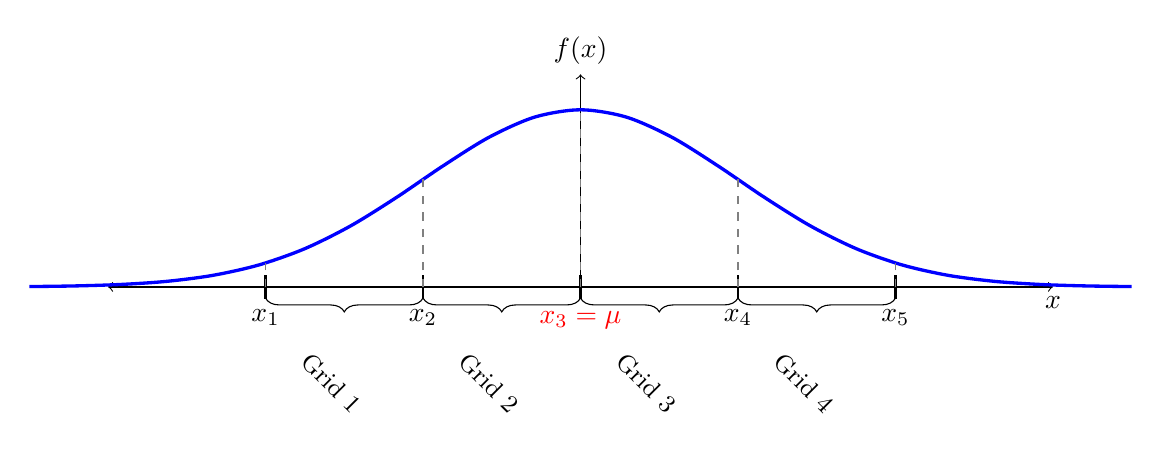
\begin{tikzpicture}[
    % Set a scale for better visibility
    xscale=2, yscale=1.5
]



% --- Define Parameters ---
\def\mean{0}      % Set mean to 0 for simplicity
\def\stdev{1}     % Standard deviation for the normal curve shape
\def\gridstep{1} % Distance between grid points (e.g., 1 * stdev)

% --- Define Grid Points ---
% 5 points are needed to create 4 segments (2 on each side of the mean)
\pgfmathsetmacro{\xone}{\mean - 2*\gridstep}
\pgfmathsetmacro{\xtwo}{\mean - 1*\gridstep}
\pgfmathsetmacro{\xthree}{\mean}
\pgfmathsetmacro{\xfour}{\mean + 1*\gridstep}
\pgfmathsetmacro{\xfive}{\mean + 2*\gridstep}

% --- Draw Axes ---
% X-axis
\draw [<->] (\mean - 3.0*\gridstep, 0) -- (\mean + 3.0*\gridstep, 0) node[below] {$x$};
% Y-axis (optional, for context)
\draw [->] (0, 0) -- (0, 1.8) node[above] {$f(x)$};

% --- Draw Normal Distribution Curve ---
% We use exp(-x^2 / (2*stdev^2)). 
% The '1.5' is a scaling factor for the height to make it look good.
\draw[blue, very thick, domain=\mean - 3.5*\stdev:\mean + 3.5*\stdev, smooth] 
    plot (\x, {1.5 * exp(-(\x - \mean)^2 / (2 * \stdev^2))});
    
% --- Mark Grid Points on X-Axis ---
% Draw tick marks and labels for the 5 grid points
\draw[thick] (\xone, 0.1) -- (\xone, -0.1) node[below] {$x_1$};
\draw[thick] (\xtwo, 0.1) -- (\xtwo, -0.1) node[below] {$x_2$};
\draw[thick] (\xthree, 0.1) -- (\xthree, -0.1) node[below, yshift=-1pt] {\textcolor{red}{$x_3=\mu$}};
\draw[thick] (\xfour, 0.1) -- (\xfour, -0.1) node[below] {$x_4$};
\draw[thick] (\xfive, 0.1) -- (\xfive, -0.1) node[below] {$x_5$};

% --- Show Discretization ---
% Draw dashed lines from grid points up to the curve
\foreach \xpos in {\xone, \xtwo, \xthree, \xfour, \xfive}
{
    \pgfmathsetmacro{\yval}{1.5 * exp(-(\xpos - \mean)^2 / (2 * \stdev^2))}
    \draw[gray, dashed] (\xpos, 0) -- (\xpos, \yval);
}

% --- Label the Segments ---
% Use braces to clearly show the 4 segments
% Segment 1 (Left)
\draw[decorate, decoration={brace, amplitude=5pt, raise=4pt,mirror}] (\xone, 0) -- (\xtwo, 0) 
    node[midway, below, yshift=-30pt,rotate=-45] {\small Grid 1};
% Segment 2 (Left)
\draw[decorate, decoration={brace, amplitude=5pt, raise=4pt,mirror}] (\xtwo, 0) -- (\xthree, 0) 
    node[midway, below, yshift=-30pt,rotate=-45] {\small Grid 2};
% Segment 3 (Right)
\draw[decorate, decoration={brace, amplitude=5pt, raise=4pt,mirror}] (\xthree, 0) -- (\xfour, 0) 
    node[midway, below, yshift=-30pt,rotate=-45] {\small Grid 3};
% Segment 4 (Right)
\draw[decorate, decoration={brace, amplitude=5pt, raise=4pt,mirror}] (\xfour, 0) -- (\xfive, 0) 
    node[midway, below, yshift=-30pt,rotate=-45] {\small Grid 4};
    
\end{tikzpicture}
\caption{Tauchen discretisation.}
\label{fig:a2_tauchen}
\end{figure}

\colorbox{Cerulean!25}{\textbf{\textit{\underline{Step 2}}} Tauchen discretisation: } \texttt{fnTauchenLogNormal} allows for conducting a quick Tauchen discretisation under the assumption that $z$ follows $\log \mathcal{N}\left(0, \sigma_z \right)$, as visualised on Figure \ref{fig:a2_tauchen}.
\\

\colorbox{Cerulean!25}{\textbf{\textit{\underline{Step 3}}} Probabilistic labour supply decision: } 
Given the presence of the Gumbel \say{shock} in the participation decision, the conditional decisions to participate, $d_v$ and $d_s$, are governed by the following binary probabilities:
\begin{subequations}
    \begin{align}
        & \mathbb{P} \left( d_v = 1 \right) = \frac{\exp \left( \frac{W}{\zeta} \right)}{\exp \left( \frac{W}{\zeta} \right)+\exp \left( \frac{N}{\zeta} \right)}
    \end{align}
    and 
    \begin{align}
        & \mathbb{P} \left( d_s = 1 \right) = \frac{\exp \left( \frac{\varphi W + (1-\varphi)N - \phi}{\zeta} \right)}{\exp \left( \frac{\varphi W + (1-\varphi)N - \phi}{\zeta} \right)+\exp \left( \frac{N}{\zeta} \right)}.
    \end{align}
\end{subequations}



